\documentclass[twoside,twocolumn]{article}

\usepackage{blindtext} % Package to generate dummy text throughout this template 
\usepackage{graphicx}
\usepackage[sc]{mathpazo} % Use the Palatino font
\usepackage[T1]{fontenc} % Use 8-bit encoding that has 256 glyphs
\linespread{1.05} % Line spacing - Palatino needs more space between lines
\usepackage{microtype} % Slightly tweak font spacing for aesthetics

\usepackage[english]{babel} % Language hyphenation and typographical rules

\usepackage[hmarginratio=1:1,top=32mm,columnsep=20pt]{geometry} % Document margins
\usepackage[hang, small,labelfont=bf,up,textfont=it,up]{caption} % Custom captions under/above floats in tables or figures
\usepackage{booktabs} % Horizontal rules in tables

\usepackage{lettrine} % The lettrine is the first enlarged letter at the beginning of the text

\usepackage{enumitem} % Customized lists
\setlist[itemize]{noitemsep} % Make itemize lists more compact

\usepackage{abstract} % Allows abstract customization
\renewcommand{\abstractnamefont}{\normalfont\bfseries} % Set the "Abstract" text to bold
\renewcommand{\abstracttextfont}{\normalfont\small\itshape} % Set the abstract itself to small italic text

\usepackage{titlesec} % Allows customization of titles
\renewcommand\thesection{\Roman{section}} % Roman numerals for the sections
\renewcommand\thesubsection{\roman{subsection}} % roman numerals for subsections
\titleformat{\section}[block]{\large\scshape\centering}{\thesection.}{1em}{} % Change the look of the section titles
\titleformat{\subsection}[block]{\large}{\thesubsection.}{1em}{} % Change the look of the section titles

\usepackage{fancyhdr} % Headers and footers
\pagestyle{fancy} % All pages have headers and footers
\fancyhead{} % Blank out the default header
\fancyfoot{} % Blank out the default footer
\fancyhead[C]{Frameworks de pruebas $\bullet$ Octubre 2021 } % Custom header text
\fancyfoot[RO,LE]{\thepage} % Custom footer text

\usepackage{titling} % Customizing the title section

\usepackage{hyperref} % For hyperlinks in the PDF
% Keywords command
\providecommand{\keywords}[1]
{
  \small	
  \textbf{\textit{Keywords---}} #1
}

%----------------------------------------------------------------------------------------
%	TITLE SECTION
%----------------------------------------------------------------------------------------
\begin{document}
\begin{titlepage}
\begin{center}
\large{UNIVERSIDAD PRIVADA DE TACNA}\\
\vspace*{-0.025in}
\begin{figure}[htb]
\begin{center}
	
\includegraphics[width=5cm]{./imagenes/logo.jpg} 
\end{center}
\end{figure}
\vspace*{0.15in}
INGENIERIA DE SISTEMAS  \\

\vspace*{0.5in}
\begin{large}
\textbf{TITULO:}\\
\end{large}

\vspace*{0.1in}
\begin{Large}
TRABAJO ENCARGADO N° 01: FRAMEWORKS DE PRUEBAS \\
\end{Large}

\vspace*{0.3in}
\begin{Large}
\textbf{CURSO:} \\
\end{Large}

\vspace*{0.1in}
\begin{large}
CALIDAD Y PRUEBAS DE SOFTWARE\\
\end{large}

\vspace*{0.3in}
\begin{Large}
\textbf{DOCENTE:} \\
\end{Large}

\vspace*{0.1in}
\begin{large}
 Patrick Cuadros Quiroga\\
\end{large}

\vspace*{0.2in}
\vspace*{0.1in}
\begin{large}
Integrantes: \\
\begin{flushleft}
Anahua Huayhua, Jenny Karen		\hfill	(2018062150) \\
Coloma Colquehuanca, Kiara Estefani		\hfill	(2018062218) \\
Cuadros Napa, Raul Marcelo         	\hfill	(2017057851) \\
Limache Durand, Rodrigo Jeral      	\hfill	(2017059278) \\
Vilca Condori, Erlang Fernando
\hfill	(2019064024) \\
\end{flushleft}
\end{large}
\vspace*{0.8in}
Tacna - Peru\end{center}
\begin{center}
2021\end{center}
\end{titlepage}
\setlength{\droptitle}{-4\baselineskip} % Move the title up
\pretitle{\begin{center}\Huge\bfseries} % Article title formatting
\posttitle{\end{center}} % Article title closing formatting
\title{Frameworks de Pruebas} % Article title
\author{Jenny Anahua, Kiara Coloma, Raul Cuadros, Rodrigo Limache y Erlang Vilca}
\date{\today} % Leave empty to omit a date
\renewcommand{\maketitlehookd}{%
\begin{large}
\centering Resumen\\
\end{large}
\vspace{0.5cm}
\noindent Un desarrollo de software contempla diferentes fases. Desde su planificación inicial, pasando por su desarrollo a su liberación oficial. Cada parte tiene su proceso, tiempos y costes y una de las que más tiempo llevan es la parte de testeo y resolución de errores. Por tanto,si estás pensando en la automatización como solución estás en el buen camino. Además, si estás pensando en crear tu propio marco de automatización de pruebas mejor es pensarlo dos veces pues en la mayoría de los casos es preferible considerar una o más de las opciones de código abierto disponibles.
\begin{abstract}
\noindent A software development contemplates different phases. From its initial planning, through its development to its official release. Each part has its own process, times and costs and one of the most time consuming is the testing and error resolution part. Therefore, if you are thinking of automation as a solution, you are on the right track. Also, if you are thinking of creating your own test automation framework, it is better to think twice, since in most cases it is preferable to consider one or more of the open source options available. 
\end{abstract}
\keywords{Frameworks, API testing, Pruebas de APIs, Software}
}
%----------------------------------------------------------------------------------------


% Print the title
\maketitle
%----------------------------------------------------------------------------------------
%	ARTICLE CONTENTS
%----------------------------------------------------------------------------------------
\section{Introduccion}

\lettrine[nindent=0em,lines=3]{U}n framework es un entorno de trabajo que tiene como objetivo facilitar la labor de programación ofreciendo una serie de características y funciones que aceleran el proceso, reducen los errores, favorecen el trabajo colaborativo y consiguen obtener un producto de mayor calidad.
Los framework ofrecen una estructura para el desarrollo y no tienen que estar sujetos a un único lenguaje de programación, aunque es habitual encontrar en el mercado, distintos frameworks específicos para un lenguaje concreto.

%------------------------------------------------
\section{Objetivos}

\begin{itemize}
\item Comparar Frameworks de Pruebas de APIs.
\item Profundizar sobre el conceptos relacionados.
\item Realizar ejemplos usando herramientas API Testing.
\end{itemize}
%------------------------------------------------
\section{Desarrollo}
\subsection{API}
Las API (Application Programming Interfaces) son un conjunto de comandos, funciones y protocolos que permiten la comunicación entre softwares.
\begin{center}
	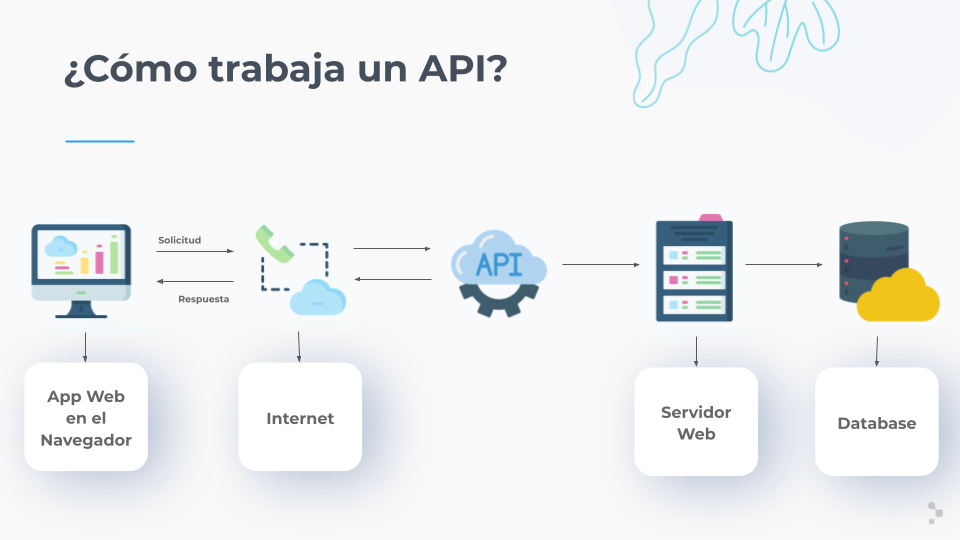
\includegraphics[width=7cm]{./imagenes/api.png} 
	\end{center}
\subsection{SOAP y REST}
SOAP es un protocolo diseñado para poder facilitar la comunicación entre plataformas, basado en XML y en otro lenguaje denominado WSDL. Del mismo modo, REST es una arquitectura más moderna y liviana, y es la más común en la que se prueba actualmente.

El hecho de que la arquitectura REST utilicé lenguaje JSON la hace más reducida y fácil de utilizar. Una gran ventaja de REST es que tiene operaciones bien definidas como son GET, POST, PUT, PATH y DELETE, siendo estas las más comunes y que detallamos a continuación..
\subsection{Metodos HTTP}
\begin{center}
	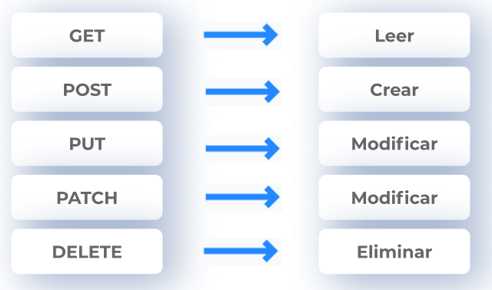
\includegraphics[width=7cm]{./imagenes/metodos.png} 
	\end{center}
\subsection{Web Services}
Los Web Services son un conjunto de estándares y protocolos para intercambiar datos entre aplicaciones. Un Web Service es una API pero que se ofrece solamente a través de internet, o sea de HTTP; en cambio las API pueden utilizar cualquier otro protocolo de comunicación.
\subsection{API Testing}
\begin{center}
	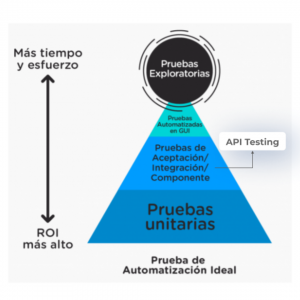
\includegraphics[width=6cm]{./imagenes/piramide.png} 
	\end{center}
De acuerdo a la Pirámide de Automatización, API Testing es un tipo de prueba de software que está dentro de los tipos de pruebas de integración.
Lo que hace API Testing es validar y verificar que las funcionalidades responden correctamente, por lo que se considera un tipo de prueba a bajo nivel, es decir, que no interactúa directamente con la interfaz de usuario.
En el caso de que estemos probando una API REST, cuando interactuamos con un Web Services por HTTP, ¿cómo sabemos que los resultados son correctos? Básicamente, por las respuestas de los códigos de estado cuando consultan información a la API.
El flujo consiste en enviar los datos de entrada, la API REST la procesa y se obtiene como resultado la salida con los siguientes códigos de respuesta:
\begin{itemize}
    \item Códigos 200: cuando son respuestas exitosas
    \item Códigos 300: cuando son mensajes de redirección
    \item Códigos 400: cuando son errores del cliente
    \item Códigos 500: cuando existen problemas con el servidor
\end{itemize}
\subsection{Beneficios de API Testing}
\begin{itemize}
    \item Promueve el Shift Left Testing,no es necesario tener el producto terminado para probar las funcionalidades.
    \item Mantenimiento sencillo
    \item Mayor velocidad de ejecucion
    \item Reduccion de errores
    \item Integracion del trabajo
\end{itemize}
\subsection{Tipos de Pruebas API}
\begin{itemize}
\item Pruebas Funcionales\\
En este tipo de pruebas se validan las funcionalidades de la API, por ejemplo al contar con una API REST, primero se validan los códigos de estado para saber que la API se encuentra disponible. También es posible validar las operaciones dependiendo de los casos de prueba, aunque no siempre es recomendable confiar en las pruebas de interfaz de usuario, por lo que realizar uno que otro flujo a nivel de API permite validar el correcto funcionamiento.

\item Pruebas de Seguridad\\
Para estas pruebas es posible probar la autenticación, si utiliza algún tipo de key o token, verificar que no cualquiera pueda utilizar la API, verificar si hay datos sensibles encriptados, entre otras aspectos. Lo anterior es lo más básico que se debe verificar en cuanto a seguridad. Otra opcion mas avanzada seria aplicar el Top 10 API Security de OWASP. 

\item Pruebas de Rendimiento\\
En este punto aparecen distintos tipos de pruebas de rendimiento, tales como: pruebas de carga, pruebas de estrés, pruebas de escalabilidad, pruebas de volumen, etc. Estas pruebas sirven para validar la carga de usuarios y que la API pueda responder correctamente a dicha carga.

\item Pruebas de Integración\\
Para validar la integración, podemos hacerlo verificando la integración con otras API integradas en un mismo proyecto.

\item Documentación\\
La documentación es muy importante al momento de probar; no podemos comenzar a probar APIs si no tenemos documentación asociada a ella. Contar con documentación representa un significativo ahorro de tiempo y esfuerzo, tanto para el tester como para el desarrollador.
\end{itemize}
\subsection{Herramientas para API Testing}
\begin{itemize}
\item SoapUI
\begin{center}
	
\includegraphics[width=6cm]{./imagenes/soapui.png} 
	\end{center}
Es una herramienta desarrollada en Java que inicialmente se utilizaba para probar servicios SOAP pero que luego se extendió para los servicios REST. Si bien SoapUI cuenta con una versión pagada, la versión gratuita contiene todo lo necesario para probar, se puede integrar con scripts de pruebas con lenguaje Groovy, y en definitiva es una de las herramientas más poderosas en el mercado.

Sin embargo, no es una herramienta muy intuitiva, en especial para aquellos que están iniciándose en el mundo del API testing, por lo que va a ser necesario requerir algún curso o tutorial guiado sobre cómo utilizarla.
\\
\item Postman
\begin{center}
	
\includegraphics[width=6cm]{./imagenes/postman.png} 
	\end{center}
Es una herramienta que principalmente se utiliza para probar API de tipo REST. Postman es una herramienta muy completa que además de probar, documentar y ayudar incluso en el proceso de desarrollo de APIs, sirve para automatizar: se pueden agregar scripts de prueba en lenguaje JavaScript.

Una de las ventajas de Postman frente a SoapUI, es que su interfaz de usuario es mucho más amigable e intuitiva, dispone de colecciones y agrupaciones de peticiones, lo que la hacen más simple de entender, incluso para aquellos que están recién comenzando.
\\
\item JMeter
\begin{center}
	
\includegraphics[width=6cm]{./imagenes/jmeter.png} 
	\end{center}
la herramienta líder para probar performance, y que es ampliamente utilizada para probar API REST. JMeter emplea múltiples lenguajes de programación y es de código abierto, por lo que se puede integrar con otras plataformas para hacer las pruebas de performance mucho más robustas.
\\
\item Rest Assured
\begin{center}
	
\includegraphics[width=6cm]{./imagenes/rest.png} 
	\end{center}
Es un framework escrito en Java que se utiliza principalmente para probar servicios REST escritos en Json o XML. La mayor ventaja que tiene Rest Assured es que al ser un framework se puede integrar con las librerías de pruebas más utilizadas, tales como JUnit, TestNG o maven. Para quienes cuentan con mayores conocimientos en programación, es una herramienta sencilla de usar y en la web hay bastante documentación.
\item Rest Client
\begin{center}
	
\includegraphics[width=4cm]{./imagenes/restclient.png}
	\end{center}
Rest Client permite enviar una solicitud HTTP y ver la respuesta en Visual Studio Code directamente.\\
Algunas de las características y ventajas que se pueden destacar de REST Client son:\\
- Ejecutar solicitudes HTTP y ver la respuesta directamente en el panel\\
- Tener todas las solicitudes en un mismo fichero\\
- Soporta los tipos de autenticación más comunes\\
- Definición de variables de entorno\\
- Generar code snippets\\
\end{itemize}
\section{Ejemplos}
Usando Postman:
\begin{center}
	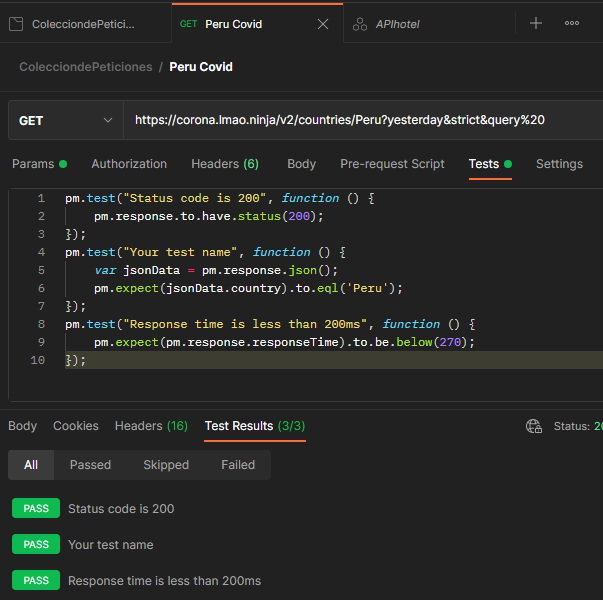
\includegraphics[width=8cm]{./imagenes/test1.png} 
	\end{center}
Usando Rest Client de Visual Studio Code:
metodo GET
\begin{center}
	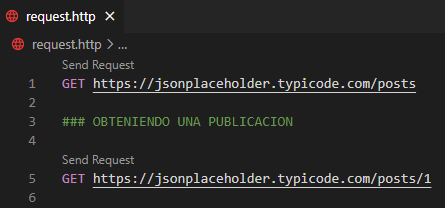
\includegraphics[width=6cm]{./imagenes/1.png} 
	\end{center}
metodo POST
\begin{center}
	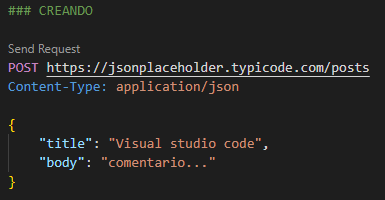
\includegraphics[width=6cm]{./imagenes/2.png} 
	\end{center}
metodo DELETE
\begin{center}
	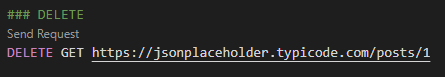
\includegraphics[width=6cm]{./imagenes/3.png} 
	\end{center}
metodo UPDATE
\begin{center}
	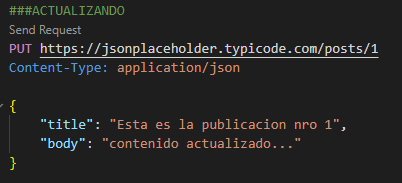
\includegraphics[width=6cm]{./imagenes/4.png} 
	\end{center}
usando variable 
\begin{center}
	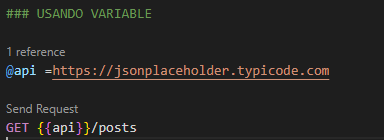
\includegraphics[width=6cm]{./imagenes/5.png} 
	\end{center}

\section{Comparativa - Rest Client & Postman}
\subsection{Postman}
- Postman es una aplicación separada que debe descargarse e instalarse, y está separada del editor de texto / IDE usado para el desarrollo (suponiendo que sea VS Code). Esto requiere un cambio de contexto un poco tedioso.\\\\
- Si está trabajando solo en un proyecto, el nivel gratuito de Postman puede ser suficiente, ya que no es necesario compartir colecciones con nadie más. Sin embargo, si trabaja en un equipo, será necesario poder compartir colecciones de solicitudes HTTP y la configuración de entornos para probar su API. Esto requiere una cuenta de Teams paga en Postman. Si se trata de una API interna o algo patentado que se está construyendo para un cliente, esto significa confiar en un tercero (Postman, la empresa) con la API y la información del entorno.\\\\
- Muchas API requieren autenticación, como un nombre de usuario / contraseña o un token proporcionado en cada solicitud. Cuando se usa Postman, esto se guarda como parte de la solicitud (o el entorno si se usan variables). Para un proyecto paralelo personal, esto puede no ser un gran problema. Pero cuando se trabaja en un proyecto de la empresa, esto convierte a Postman en un administrador de secretos.
\subsection{Rest Client}
- En Rest client el uso de las solicitudes http no requiere salir del editor.Puede usar las teclas de acceso directo habituales para encontrar los archivos http, intellisense en las variables de entorno al editar los archivos http, e incluso admite la búsqueda de solicitudes por símbolo, al igual que cualquier otro archivo de código en VS Code.\\\\
- Los archivos .http son parte de su proyecto, por lo tanto, viven bajo el mismo control de versión que el resto de su código. Ahora obtiene todos los beneficios de las revisiones de git y relaciones públicas, y las solicitudes están vinculadas al código que están probando. 

\section{Conclusiones}
Independientemente, habría la misma funcionalidad accesible en todas las herramientas API, pero el enfoque es diferente. La mejor manera de experimentarlos es intentarlo para ver qué funciona mejor para los requisitos de su negocio.\\
Podemos concluir que sin importar la herramienta de automatización que estemos utilizando, es importante que por medio de las metodologías anteriormente mencionadas, la integremos en algún framework para así tener todos los beneficios de la misma en lo que queramos automatizar.
\section{Recomendaciones}
Presentadas todas estas opciones llega el momento de elegir una. En realidad no hay un claro ganador, el presente artículo no pretende crear un ranking de framework para testing automation sino enumerar alguna de las múltiples opciones basadas en código abierto disponibles. 
Quizá el mejor consejo es que antes de escribir esa primera línea de código para crear su propio framework, asegúrate de que no haya una biblioteca o framework existente que puedas aprovechar. Deja de perder el tiempo reinventando la rueda; Echa un vistazo a estos framework de automatización primero.

%----------------------------------------------------------------------------------------
%	REFERENCE LIST
%----------------------------------------------------------------------------------------

\begin{thebibliography}{99}
	\bibitem - Aguilera, Cecilia. (2021). API Testing: Guía práctica para iniciarse. Blog de Testing y Calidad de Software | Abstracta Chile.

    \bibitem - Parada, Miguel. (2020). 6 Frameworks abiertos para testing automation. OpenExpo Virtual Experience 2021.

    \bibitem - Aldaine, Alice. (2021). Top 10 API Testing Tools in 2020 (Detailed Reviews). Medium.

    \bibitem - Naini, Anjaneyulu. (2020). Las 11 mejores herramientas para probar y construir API más rápido. Geekflare.

    \bibitem - Veskovic, Nemanja. (2018). REST Assured vs. JMeter: Una comparación de las Herramientas de Prueba de REST. Toptal Engineering Blog.

    \bibitem - Josepablosarco. (2018). Top 7 Frameworks de Pruebas Automatizadas. Testing en Español.

    \bibitem - Zabolennyi, Serhii. (2021). Karate Framework: Testeo de APIs de Impacto. Apiumhub.

    \bibitem - Ciberninjas. (2021). Las 11 Mejores Herramientas de Automatización de Pruebas para Interfaces de Usuario 2021. Ciberninjas.
	\end{thebibliography}

%----------------------------------------------------------------------------------------

\end{document}
